\subsection{Grundlagen}
Vom Ultraschall wird gesprochen, wenn sich Frequenzen in einem Bereich von
$20\kHz$ bis $1\GHz$ befinden. Der für Menschen hörbare Bereich liegt zwischen
$16\Hz$ und $20\kHz$. Der Bereich über dem Ultraschall wird als Hyperschall und
der Bereich unter dem hörbaren Bereich als Infraschall bezeichnet.

Eine Änderung der Frequenz, wenn sich eine Frequenzquelle und ein Beobachter
relativ zueinander bewegen ist als Doppler-Effekt bekannt. Wenn sich die Quelle
auf den Beobachter zu bewegt, wird die Frequenz $\nu_0$ in einen höheren
Frequenzbereich $\nu_+$ verschoben. Entfernt sich die Quelle vom Beobachter,
wird $\nu_0$ in einen kleineren Bereich $\nu_-$ verschoben. Allgemein lässt
sich die neue Frequenz mit
\begin{equation}
  \nu_\pm = \frac{\nu_0}{1\mp\frac{v}{c}}
\end{equation}
berechnen. Hierbei ist $v$ die Geschwindigkeit der Quelle und $c$ die
Schallgeschwindigkeit im Medium.
Bewegt sich der Beobachter und die Quelle ruht, wird die neue Frequenz mit
\begin{equation}
  \nu_\pm=\nu_0\left(1\pm\frac{v}{c}\right)
\end{equation}
berechnet. In der Ultraschalltechnik wird der Doppler-Effekt genutzt um die
Geschwidigkeiten von Blutströmungen zu bestimmen. Trifft eine Ultraschallwelle
auf ein bewegtes Objekt, wie etwa einen Blutkörper, verschiebt sich die Frequenz
gemäß Doppler-Effekt.
\begin{wrapfigure}{r}{5cm}
  \centering
  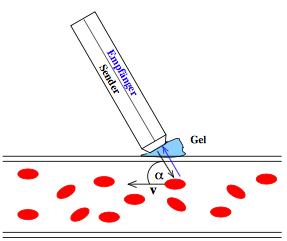
\includegraphics[width=4cm]{bilder/sender.png}
  \caption{Sender und Empfänger mit gleichem Einstrahl-/Empfangswinkel \cite{us3}.}
\end{wrapfigure}
Neben der Geschwindigkeit des Objektes und der
Schallgeschwindigkeit hängt die Verschiebung auch von den Winkeln $\alpha$ und
$\beta$ zwischen der Geschindigkeit $v$ und der Wellennormalen der einlaufenden
bzw auslaufenden Welle ab. Bei dem verwendeten Impul-Echo-Verfahren sind beide
Winkel identisch, sodass für die Frequenzverschiebung gilt:
\begin{equation}
  \Delta\nu = 2\nu_0\frac{v}{c}\cos(\alpha).
  \label{eqn:deltanu}
\end{equation}
Der Doppler-Winkel $\alpha$ hängt von dem Prismenwinkel $\theta$, der
Schallgeschwindigkeit im Prismamaterial $c_\su{p}$ und der Schallgeschwindigkeit
der Dopplerflüssigkeit $c_\su{L}$ ab. Sind alle Parameter bekannt, lässt sich
der Doppler-Winkel mit
\begin{equation}
  \alpha = 90\dgr -\arcsin\left(\sin\theta\,\frac{c_\su{L}}{c_\su{p}}\right)
  \label{eqn:alpha}
\end{equation}
berechnen.
\subsection{Erzeugung von Ultraschall-Wellen}
Ultraschall-Wellen lassen sich mit Hilfe des piezo-elektrischen Effekt erzeugen.
Hierbei wird ein piezoelektrischer Kristall in ein elektrisches Wechselfeld
gebracht und zu Schwingungen angeregt. Durch die Schwingung des Kristalls werden
Ultraschallwellen erzeugt. Um möglichst hohe Schallenergiedichten zu erhalten,
muss die Resonanz erreicht werden was zu großen Schwingungsamplituden führt.
Der Piezokristall kann zudem auch als Empfänger genutzt werden. Hierbei treffen
Schallwellen auf den Kristall und regen diesen wiederum zu Schwingungen an.

Häufig werden Quarze als piezoeletrische Kristalle verwendet, da diese
gleichbleibende physikalische Eigenschaften besitzen. Jedoch besitzen sie nur
einen sehr schwachen piezoelektrischen Effekt.
